%$Header: svn://localhost/dtapublic/pubs/books/ucbka/trunk/c_fry0/c_fry0.tex 277 2019-08-13 02:35:39Z dashley $

\chapter{\cfryzerolongtitle{}}

\label{cfry0}

\beginchapterquote{``\ldots{} Beauty is the first test:  there is no permanent
                   place in the world for ugly mathematics.''}
                   {G. H. Hardy \cite[p.85]{bibref:b:mathematiciansapology:1940}}
				   \index{Hardy, G. H.}

\section{Introduction}
%Section Tag: INT
\label{cfry0:sint}

The \emph{Farey series
of order $N$},\index{Farey series} denoted $F_{N}$,\index{F@$F_N$}
is the ordered set of all irreducible
rational numbers $h/k$ in the interval
[0,1]
with denominator $k\leq N$.
As examples, the Farey series of
orders 1 through 7, $F_1$ through $F_7$, are shown
in (\ref{eq:cfry0:sint:eq0001a}) through (\ref{eq:cfry0:sint:eq0001g}).

\begin{equation}
\label{eq:cfry0:sint:eq0001a}
F_1  = \left\{ {\frac{0}{1},\frac{1}{1}} \right\}
\end{equation}

\begin{equation}
\label{eq:cfry0:sint:eq0001b}
F_2  = \left\{ {\frac{0}{1},\frac{1}{2},\frac{1}{1}} \right\}
\end{equation}

\begin{equation}
\label{eq:cfry0:sint:eq0001c}
F_3  = \left\{ {\frac{0}{1},\frac{1}{3},\frac{1}{2},
                \frac{2}{3},\frac{1}{1}} \right\}
\end{equation}

\begin{equation}
\label{eq:cfry0:sint:eq0001d}
F_4  = \left\{ {\frac{0}{1},\frac{1}{4},
                \frac{1}{3},\frac{1}{2},
                \frac{2}{3},\frac{3}{4},
                \frac{1}{1}} \right\}
\end{equation}

\begin{equation}
\label{eq:cfry0:sint:eq0001e}
F_5  = \left\{ {\frac{0}{1},\frac{1}{5},\frac{1}{4},
                \frac{1}{3},\frac{2}{5},\frac{1}{2},
                \frac{3}{5},\frac{2}{3},\frac{3}{4},
                \frac{4}{5},\frac{1}{1}} \right\}
\end{equation}

\begin{equation}
\label{eq:cfry0:sint:eq0001f}
F_6  = \left\{ {\frac{0}{1},\frac{1}{6},\frac{1}{5},
                \frac{1}{4},
                \frac{1}{3},\frac{2}{5},\frac{1}{2},
                \frac{3}{5},\frac{2}{3},
                \frac{3}{4},
                \frac{4}{5},
                \frac{5}{6},\frac{1}{1}} \right\}
\end{equation}


\begin{equation}
\label{eq:cfry0:sint:eq0001g}
F_7  = \left\{ {\frac{0}{1},\frac{1}{7},\frac{1}{6},\frac{1}{5},
                \frac{1}{4},\frac{2}{7},
                \frac{1}{3},\frac{2}{5},\frac{3}{7},\frac{1}{2},
                \frac{4}{7},\frac{3}{5},\frac{2}{3},
                \frac{5}{7},\frac{3}{4},
                \frac{4}{5},
                \frac{5}{6},\frac{6}{7},\frac{1}{1} } \right\}
\end{equation}


The distribution of Farey rational numbers in
[0,1] is repeated
in any
$[i,i+1]$, $i\in \vworkintset$; so that the distribution of
Farey rationals in [0,1] supplies complete
information about the distribution in
all of $\vworkrealset$.  We
occasionally abuse the proper nomenclature by referring
to sequential rational numbers outside the
interval [0,1] as Farey terms or as part of
$F_N$, which, technically, they are not.
All of the results presented in
this chapter, with the exception of results concerning the number
of terms, can be shown to apply
everywhere in $\vworkrealsetnonneg$, so this abuse
is not harmful.

The study of the Farey series is a topic from number theory
(a branch of mathematics).  The Farey series finds application
in microcontroller work because very often it is economical
to linearly scale an integer $x$ using a rational approximation
of the form $\lfloor hx/k \rfloor$, $h \in \vworkintsetnonneg$,
$k \in \vworkintsetpos$ (a single integer multiplication followed by
a single integer division with the remainder discarded).
The economy of this type of linear scaling comes about because
many microcontrollers have integer multiplication and division
instructions.  However, the technique requires that we be
able to choose $h$ and $k$ so as to place $h/k$ as close
as possible to the real number $r_I$ that we wish to
approximate; always subject to the constraints
$h \leq{} h_{MAX}$ and $k \leq k_{MAX}$ (since microcontroller
multiplication and division instructions are constrained in
the size of the operands they can accomodate).

Without the relevant results from number theory, it is
very difficult to find the rational numbers $h/k$:
$h \in \vworkintsetnonneg, \leq{} h_{MAX}$, $k \in \vworkintsetpos, \leq k_{MAX}$
closest to
an arbitrary $r_I \in \vworkrealsetnonneg$, even for moderate
choices of $h_{MAX}, k_{MAX}$ (see Example \ref{ex:cfry0:sint:01}).
A poorly-written brute-force
algorithm might iterate over all $h$ and all $k$ to find the
rational numbers closest to $r_I$; and thus might be
approximately $O(h_{MAX} k_{MAX})$.  A refined brute-force
algorithm might refine the search and be approximately
$O(min(h_{MAX}, k_{MAX}))$.  However, for implementation on powerful
computers which have machine instructions to multiply and
divide large integers, or for extended-precision integer arithmetic, even algorithms
which are $O(min(h_{MAX}, k_{MAX}))$ are not  practical.  The best
algorithm presented in this work (utilizing the
framework of continued fractions), is $O(log \; max(h_{MAX}, k_{MAX}))$,
and so is practical even for very large $h_{MAX}$ and $k_{MAX}$.

\begin{vworkexamplestatement}
\label{ex:cfry0:sint:01}
Find the rational numbers
$h/k$ which enclose $1/e \approx 0.3678794412$
subject to the constraint $k \leq 2^{16} - 1 = 65\vworkthousandsdigsepinmathmode{}535$.%
\footnote{This example is intended to demonstrate the difficulty of
finding suitable rational numbers near an arbitrary $r_I$ without the
relevant results from number theory.}
\end{vworkexamplestatement}
\begin{vworkexampleparsection}{Solution}
$1/e$ is irrational, and so has left and right neighbors in
the Farey series of any order.  Using algorithms that will be presented later in the
work, these two enclosing rational numbers subject to the
constraint $k \leq 2^{16}-1$ are
$18\vworkthousandsdigsepinmathmode{}089/49\vworkthousandsdigsepinmathmode{}171$
and
$9\vworkthousandsdigsepinmathmode{}545/25\vworkthousandsdigsepinmathmode{}946$.
\end{vworkexampleparsection}
\vworkexamplefooter{}

%%%%%%%%%%%%%%%%%%%%%%%%%%%%%%%%%%%%%%%%%%%%%%%%%%%%%%%%%%%%%%%%%%%%%%%%%%%%%%
%%%%%%%%%%%%%%%%%%%%%%%%%%%%%%%%%%%%%%%%%%%%%%%%%%%%%%%%%%%%%%%%%%%%%%%%%%%%%%
%%%%%%%%%%%%%%%%%%%%%%%%%%%%%%%%%%%%%%%%%%%%%%%%%%%%%%%%%%%%%%%%%%%%%%%%%%%%%%
\section{History Of The Farey Series}
%Section tag:  HFS

\index{Farey series!history of}
The Farey series owes its name to John Farey,
\index{Farey, John} a British geologist who in 1816
published the statement to the effect that in the Farey series the middle
of any three consecutive terms is the mediant of the other two
\cite{bibref:w:CutTheKnotMainPage}\footnote{\label{fn:cfry0:hfs01}Exact URL:
\texttt{http://www.cut-the-knot.com/blue/FareyHistory.html}.} (Thm.
\ref{thm:cfry0:spfs:03} in this work).
However, many mathematicians
believe that credit for the Farey series is misplaced, and that the
series should not have been named after Farey.  In
\emph{A Mathematician's Apology} 
\cite[pp. 81-82]{bibref:b:mathematiciansapology:1940},
Hardy cites the Farey series as one of the rare examples in scientific
history where credit is misplaced:

\begin{indentedquote}
``\ldots{} Farey is immortal because he failed to understand a theorem
which Haros had proved perfectly fourteen years
before \ldots{} but on the whole the history of science is fair, and 
this is particularly
true in mathematics \ldots{} and the men who are remembered are almost
always the men who merit it.''
\end{indentedquote}

Hardy and Wright also provide a footnote about the history
of the Farey series, \cite[pp. 36-37]{bibref:b:HardyAndWrightClassic}:

\begin{indentedquote}
``The history of the Farey series is very curious.
Theorems 28 and 29\footnote{Theorems
\ref{thm:cfry0:spfs:02} and \ref{thm:cfry0:spfs:03},
respectively, in this chapter.} seem to have been stated and proved first by
Haros in 1802; see Dickson, \emph{History}, i. 156.
Farey did not publish anything on the subject until
1816, when he stated Theorem 29 in a note in the
\emph{Philosophical Magazine}.  He gave no proof, and it is unlikely that he
had found one, since he seems to have been at the best an
indifferent mathematician.

Cauchy, however, saw Farey's statement, and supplied the
proof (\emph{Exercices de math\'ematiques}, i. 114-116).  Mathematicians
generally have followed Cauchy's example in attributing the results to
Farey, and the results will no doubt continue to bear his name.''
\end{indentedquote}

\cite{bibref:w:CutTheKnotMainPage}$^{\ref{fn:cfry0:hfs01}}$ contains the best
account of the history of the Farey series on the Web (and contains
information on many other
interesting topics related to mathematics and number theory, as well).  At this
site, Dr. Alexander Bogomolny
\index{Bogomolny, Alexander} has included John Farey's
original letter to the \emph{Philosophical Magazine}, and much historical
and human perspective.  This site is highly recommended for anyone who has
an interest in mathematics, number theory, and history.


%%%%%%%%%%%%%%%%%%%%%%%%%%%%%%%%%%%%%%%%%%%%%%%%%%%%%%%%%%%%%%%%%%%%%%%%%%%%%%
%%%%%%%%%%%%%%%%%%%%%%%%%%%%%%%%%%%%%%%%%%%%%%%%%%%%%%%%%%%%%%%%%%%%%%%%%%%%%%
%%%%%%%%%%%%%%%%%%%%%%%%%%%%%%%%%%%%%%%%%%%%%%%%%%%%%%%%%%%%%%%%%%%%%%%%%%%%%%

\section{Properties Of Terms Of The Farey Series}
%Section tag:  PFS

\index{Farey series!properties of}
In Section \ref{cfry0:sint}, we hinted that the properties
of the Farey series (which, technically,
consists of irreducible rational numbers $h/k$
only in $[0,1]$) hold in any interval $[n,n+1]$,
$n \in \vworkintsetpos$.  We would first like to show
that if $h/k \in [0,1]$ is irreducible, then
any of its corresponding rational numbers $(h+ik)/k$ in
$[i,i+1]$, $i \in \vworkintsetpos$ are also irreducible.

\begin{vworktheoremstatement}
\label{thm:cfry0:spfs:01}
Iff $h/k$, $k \in \vworkintsetpos$, $h \in \{0, 1, \ldots{}, k\}$
is irreducible, then

\begin{equation}
\frac{h}{k} + i = \frac{h + ik}{k}
\end{equation}

is also irreducible for $i \in \vworkintsetnonneg$.
\end{vworktheoremstatement}
\begin{vworktheoremproof}
Let $\{p_k^{a_k}\} = p_1^{a_1} p_2^{a_2} \ldots{} p_M^{a_M}$ be the prime
factorization of $h$.
Let $\{q_k^{b_k}\} = q_1^{b_1} q_2^{b_2} \ldots{} q_M^{b_M}$ be the prime
factorization of $k$.  The coprimality of $h$ and $k$ ensures that
$\{p_k^{a_k}\} \bigcap \{q_k^{b_k}\} = \oslash$.  We are interested in the
irreducibility (or lack thereof) of

\begin{equation}
\label{eq:cfry0:spfs:01}
\frac{h}{k} + i =
\frac{p_1^{a_1} p_2^{a_2} \ldots{} p_M^{a_M} +
i(q_1^{b_1} q_2^{b_2} \ldots{} q_N^{b_N})}
{q_1^{b_1}  q_2^{b_2} \ldots{} q_N^{b_N}}
\end{equation}

In order for the expression in (\ref{eq:cfry0:spfs:01}) to be reducible,
it is necessary for at least one $q_k \in \{q_1, q_2, \ldots{}, q_N\}$
to divide the numerator, which is possible only if
$\{p_k\} \bigcap \{q_k\} \neq \oslash$.  (The degenerate cases
of $h=1$ or $k=1$ are left for the reader as
Exercise \ref{exe:cfry0:sexe0:01}.)
\end{vworktheoremproof}
\begin{vworktheoremparsection}{Remarks}
On the other hand, if $h/k$ is reducible, let
$\{p_k^{a_k}\} = p_1^{a_1} p_2^{a_2} \ldots{} p_M^{a_M}$
be the prime factors of $h$ which do not appear in $k$, let
$\{q_k^{b_k}\} = q_1^{b_1} q_2^{b_2} \ldots{} q_N^{b_N}$
be the prime factors of $k$ which do not appear in $h$,
and let
$\{s_k^{c_k}\} = s_1^{c_1} s_2^{c_2} \ldots{} s_L^{c_L}$
be the prime factors which appear in both $h$ and $k$.
We are interested in the irreducibility (or lack thereof)
of

\begin{equation}
\label{eq:cfry0:spfs:02}
\frac{h}{k} + i =
\frac{ \{ s_k^{c_k} \} \{ p_k^{a_k} \} + i \{ s_k^{c_k} \} \{ q_k^{b_k} \} }
{ \{ s_k^{c_k} \} \{ q_k^{b_k} \} }.
\end{equation}

It is clear that any choice of 
$i \in \vworkintsetnonneg$ will allow $\{s_k^{c_k}\}$
to divide both the numerator and the denominator.
\end{vworktheoremparsection}
\vworktheoremfooter{}

\index{rational number!comparison of}
Very frequently, it is necessary to compare rational numbers
to determine if they are equal; and if not, which is larger.
This need occurs both in symbolic manipulation (derivations and
proofs), and in calculations.  We present a property which is
useful for comparison of non-negative rational numbers.

\begin{vworklemmastatement}
\label{lem:cfry0:spfs:02b}
For $a,c \geq 0$ and $b,d > 0$,

\begin{equation}
\begin{array}{lr}
\displaystyle{\frac{a}{b} < \frac{c}{d}},      &  iff \;\; ad < bc             \\
                                               &                               \\
\displaystyle{\frac{a}{b} = \frac{c}{d}},      &  iff \;\; ad = bc             \\
                                               &                               \\
\displaystyle{\frac{a}{b} > \frac{c}{d}},      &  iff \;\; ad > bc             
\end{array}
\end{equation}
\end{vworklemmastatement}
\begin{vworklemmaproof}
Assume $a,c \geq 0$ and $b,d > 0$.
Under these assumptions, $a/b < c/d \vworkequiv a < bc/d \vworkequiv ad < bc$.
Similarly, under the same assumptions, 
$a/b = c/d \vworkequiv a = bc/d \vworkequiv ad = bc$ and
$a/b > c/d \vworkequiv a > bc/d \vworkequiv ad > bc$.
\end{vworklemmaproof}
\begin{vworklemmaparsection}{Remarks}
Note it is not required that
$a, b, c, d \in \vworkintset$, although this is the way in which
the lemma is used exclusively in this work.  Note also that the lemma does 
not cover the case when any of the components $a,b,c,d$ are $<0$.
For comparing rational numbers
\index{rational number!comparison of} 
with non-negative components, this lemma presents
the most convenient method.
\end{vworklemmaparsection}
\vworklemmafooter{}

Some properties and results concerning the Farey series rely
on the \emph{mediant}\index{mediant}\index{rational number!mediant of} 
of two rational numbers,
which is defined now.

\begin{vworkdefinitionstatementpar}{Mediant}
\label{def:cfry0:spfs:02}
The \emph{mediant} of two [irreducible] rational numbers
$h/k$ and $h'/k'$ is the [reduced form of the] fraction
\begin{equation}
\frac{h+h'}{k+k'} .
\end{equation}
\end{vworkdefinitionstatementpar}
\begin{vworkdefinitionparsection}{Remarks}
Note that the mediant of two rational numbers---even
irreducible rational numbers---is not necessarily irreducible.
For example, the mediant of 1/3 and 2/3 is 3/6, which is
not irreducible.  Note also that the mediant of two rational
numbers is ambiguously defined if we don't require that the 
rational numbers be irreducible.  For example, 
the mediant of 1/3 and 2/3 is 3/6 = 1/2, but the
mediant of 2/6 and 2/3 is 4/9 (a different number than
1/2).  Normally, in this work, we will calculate the mediant
only of irreducible rational numbers, and we will define
the result to be the reduced form of the fraction calculated.
\end{vworkdefinitionparsection}
\vworkdefinitionfooter{}

The mediant of two rational numbers always lies between them in value (but
is not necessarily the midpoint).  A somewhat stronger
statement about mediants can be made, and is 
presented as Lemma \ref{lem:cfry0:spfs:02c}, below.

\begin{vworklemmastatement}
\label{lem:cfry0:spfs:02c}
For 
$a,c \geq 0$,
$b,d,i,j > 0$, and
$a/b < c/d$,

\begin{equation}
\frac{a}{b} < \frac{ia + jc}{ib + jd} < \frac{c}{d} ,
\end{equation}

or, equivalently,

\begin{equation}
\frac{ia + jc}{ib + jd} \in \left( { \frac{a}{b} , \frac{c}{d} } \right) .
\end{equation}

\end{vworklemmastatement}
\begin{vworklemmaproof}
Under the restrictions on $a,b,c,d,i$, and $j$;
$ad < bc \vworkhimp ijad < ijbc \vworkhimp i^2ab+ijad < i^2ab + ijbc$
$\vworkhimp ia(ib+jd) < ib(ia+jc) \vworkhimp ia/ib < (ia+jc)/(ib+jd)$
(employing Lemma \ref{lem:cfry0:spfs:02b}).  A similar implication
can be used to show that $(ia+jc)/(ib+jd) < jc/jd$.
\end{vworklemmaproof}
\begin{vworklemmaparsection}{Remarks}
A special case of this lemma is the result that the mediant of two
rational numbers is always between them ($i=j=1$).  This lemma gives
some insight into the arrangement of 
intermediate fractions\index{intermediate fraction}\index{continued fraction!intermediate fraction}
between
two convergents\index{continued fraction!convergent}
(see \ccfrzeroxrefcomma{}\ccfrzeromcclass{} \ref{ccfr0}, 
\emph{\ccfrzeroshorttitle{}}).
\end{vworklemmaparsection}
%\vworklemmafooter{}

\begin{vworktheoremstatement}
\label{thm:cfry0:spfs:02ba}
If $h/k$ and $h'/k'$ are two successive terms
of $F_N$, then $k + k' > N$.
\end{vworktheoremstatement}
\begin{vworktheoremproof}
By Lemma \ref{lem:cfry0:spfs:02c}, 
the mediant of $h/k$ and $h'/k'$ lies between them, i.e.

\begin{equation}
\label{eq:cfry0:spfs:02baa}
\frac{h + h'}{k + k'} \in \left( { \frac{h}{k}, \frac{h'}{k'}} \right) .
\end{equation}

Note that if $k+k' \leq N$, the denominator of the mediant, $k+k'$, is less than
$N$, so that either the fraction specified by (\ref{eq:cfry0:spfs:02baa}) or its 
reduced form is in $F_N$; hence there is another term between $h/k$ and 
$h'/k'$ in $F_N$.  (See \cite[Thm. 30, p. 23]{bibref:b:HardyAndWrightClassic}.)
\end{vworktheoremproof}
%\vworktheoremfooter{}

\begin{vworktheoremstatement}
\label{thm:cfry0:spfs:02c}
For $N > 1$, no two consecutive terms of $F_N$ have the
same denominator.
\end{vworktheoremstatement}
\begin{vworktheoremproof}
Assume that $h/k$ and $h'/k$ are the two consecutive terms with 
the same denominator.  Note that the only choice of $h'$ which
could be the numerator of a consecutive term is $h'=h+1$; otherwise 
we would have $h/k < (h+1)/k < h'/k$, which implies that $h/k$
and $h'/k'$ are not consecutive, a contradiction.  With
$h'=h+1$ (the only possibility), let's examine the inequality $h/k < h/(k-1) < (h+1)/k$.
$h/k < h/(k-1)$ is always true for any choice of $k>1$.  
It can be shown using Lemma \ref{lem:cfry0:spfs:02b}
that $h/(k-1) < (h+1)/k$ is true iff $h < k -1$.  So,
for any $h \in \{2, \ldots{} , k - 2 \}$, we can always use
the fraction $h/(k-1)$ as an intermediate term to show that
$h/k$ and $(h+1)/k$ are not consecutive in $F_N$.
If $h=k-1$, then we are considering the two fractions
$(k-1)/k$ and $k/k$, and $k/k$ cannot be in lowest 
terms---after reducing $k/k$ the two fractions 
being considered no longer have the
same denominator. (See \cite[Thm. 31, p. 24]{bibref:b:HardyAndWrightClassic}.)
\end{vworktheoremproof}
%\vworktheoremfooter{}

\begin{vworktheoremstatement}
\label{thm:cfry0:spfs:02}
If $h/k$ and $h'/k'$ are two successive terms of $F_N$, then

\begin{equation}
\label{eq:cfry0:spfs:thm02aa}
h'k - h k' = 1.
\end{equation}
\end{vworktheoremstatement}

\begin{vworktheoremproof}
For any $h/k$, Lemma \cprizeroxrefhyphen\ref{lem:cpri0:ppn0:00a} guarantees
that an $h'/k'$ satisfying (\ref{eq:cfry0:spfs:thm02aa}) exists.
If $h'=x_0, k'=y_0$ is a solution, then
$h'=x_0 + r h, k'=y_0 + r k, r \in \vworkintset$ is also
a solution, and Lemma \cprizeroxrefhyphen\ref{lem:cpri0:ppn0:000p}
guarantees that any $h', k'$ so chosen will be coprime.
Note that $r$ can be chosen so that $0 \leq N-k < k' \leq N$, and
that h'/k' will be $\in F_N$.

However, it still needs to be established that $h'/k'$ is the
\emph{next} term in $F_N$ (i.e. that there can be no intervening
terms).  To show this, assume that an intervening term
$a/b$ exists, so that $h/k < a/b < h'/k'$, with $b \leq N$.
In this case, the distance from $h/k$ to $a/b$ is

\begin{equation}
\label{eq:cfry0:spfs:thm02ab}
\frac{a}{b}-\frac{h}{k} = \frac{ak-bh}{bk} \geq \frac{1}{bk} .
\end{equation}

Similarly, the distance from $a/b$ to $h'/k'$ is

\begin{equation}
\label{eq:cfry0:spfs:thm02ab2}
\frac{h'}{k'}-\frac{a}{b} = \frac{h'b-k'a}{k'b} \geq \frac{1}{k'b} .
\end{equation}

(The inequalities in Eqns. \ref{eq:cfry0:spfs:thm02ab}
and \ref{eq:cfry0:spfs:thm02ab2} come
about through Lemma \ref{lem:cfry0:spfs:02b}---the numerator
in each case must be at least $1$ if it is assumed 
$h/k < a/b < h'/k'$.)

The distance from $h/k$ to $h'/k'$ is

\begin{equation}
\label{eq:cfry0:spfs:thm02ac}
\frac{h'}{k'}-\frac{h}{k} = \frac{h'k-hk'}{kk'} = \frac{1}{kk'} .
\end{equation}

The distance from $h/k$ to $h'/k'$ must be the sum of the distances
from $h/k$ to $a/b$ and from $a/b$ to $h'/k'$:

\begin{equation}
\label{eq:cfry0:spfs:thm02ad}
\left( { \frac{h'}{k'} - \frac{h}{k} } \right)
=
\left( { \frac{a}{b} - \frac{h}{k} } \right)
+
\left( { \frac{h'}{k'} - \frac{a}{b} } \right) .
\end{equation}

Substituting (\ref{eq:cfry0:spfs:thm02ab}),
(\ref{eq:cfry0:spfs:thm02ab2}), 
and (\ref{eq:cfry0:spfs:thm02ac}) 
into (\ref{eq:cfry0:spfs:thm02ad}) leads 
to

\begin{equation}
\label{eq:cfry0:spfs:thm02ae}
\frac{1}{kk'}
\geq
\frac{1}{bk}+\frac{1}{k'b}
=\frac{k'}{bkk'}+\frac{k}{bkk'}
=\frac{k'+k}{bkk'}
>
\frac{N}{bkk'}
>
\frac{1}{kk'} ,
\end{equation}

a contradiction.  Therefore, $a/b$ must be $h'/k'$ and 
$h'k-hk'=1$.  (See \cite{bibref:b:HardyAndWrightClassic}, Thm. 28, p. 23,
and the second proof on pp. 25-26.)
\end{vworktheoremproof}
%\vworktheoremfooter{}

\begin{vworklemmastatement}
\label{lem:cfry0:spfs:03b}
For $h/k$, $h'/k'$ and $h''/k''$; $h, h', h'' \in \vworkintsetnonneg$, 
$k, k', k'' \in \vworkintsetpos$, with

\begin{equation}
h'k-hk' = h''k'-h'k''=1 ,
\end{equation}

\begin{equation}
(k'>k'') \vworkhimp
\left( {
\frac{h'}{k'}-\frac{h}{k}<\frac{h''}{k''}-\frac{h}{k}
} \right) .
\end{equation}
\end{vworklemmastatement}
\begin{vworklemmaproof}
\begin{equation}
\frac{h'}{k'}-\frac{h}{k} = \frac{1}{kk'}
\end{equation}
\begin{equation}
\frac{h''}{k''}-\frac{h}{k} = \frac{1}{kk''}
\end{equation}
\begin{equation}
(k' > k'') \vworkhimp \left( {
\frac{1}{kk'} < \frac{1}{kk''}
} \right)
\end{equation}
\end{vworklemmaproof}
\begin{vworklemmaparsection}{Remarks}
This lemma essentially says that if more than one potential successor to
$h/k$ in $F_N$, $h'/k'$ and $h''/k''$, both meet the necessary test
provided by Theorem \ref{thm:cfry0:spfs:02}, the potential successor
with the largest denominator is the successor, because it is closer to
$h/k$.  This lemma is used in proving Theorem \ref{thm:cfry0:sgfs0:01}.
\end{vworklemmaparsection}
%\vworklemmafooter{}

\begin{vworktheoremstatement}
\label{thm:cfry0:spfs:03}
If $h/k$, $h'/k'$, and $h''/k''$ are three successive terms of $F_N$, then

\begin{equation}
\frac{h'}{k'} = \frac{h+h''}{k+k''}.
\end{equation}
\end{vworktheoremstatement}
\begin{vworktheoremproof}
Starting from Theorem \ref{thm:cfry0:spfs:02}:
\begin{equation}
h'k-hk' = h''k' - h'k''=1
\end{equation}
\begin{equation}
h'(k+k'')=k'(h+h'')
\end{equation}
\begin{equation}
\frac{h'}{k'} = \frac{h+h''}{k+k''}.
\end{equation}
\end{vworktheoremproof}
\vworktheoremfooter{}


%%%%%%%%%%%%%%%%%%%%%%%%%%%%%%%%%%%%%%%%%%%%%%%%%%%%%%%%%%%%%%%%%%%%%%%%%%%%%
%%%%%%%%%%%%%%%%%%%%%%%%%%%%%%%%%%%%%%%%%%%%%%%%%%%%%%%%%%%%%%%%%%%%%%%%%%%%%
%%%%%%%%%%%%%%%%%%%%%%%%%%%%%%%%%%%%%%%%%%%%%%%%%%%%%%%%%%%%%%%%%%%%%%%%%%%%%
\section{Generation Of Terms Of The Farey Series}
\label{cfry0:sgfs0}
%Section tag:  GFS0


\index{Farey series!generation of terms}
Earlier sections of this chapter have enumerated important properties of the
Farey series.  However, these properties are of limited practical value
because they don't help to solve practical problems in microcontroller
work---one would like to be able to generate (in order, of course) all of
the terms of a Farey series so that one can choose suitable terms
near some $r_I \in \vworkrealsetnonneg$ that one wishes to approximate 
with $r_A = h/k$.

Fortunately, the properties presented in earlier sections do allow the
generation of successive Farey terms, as the following theorem shows.

\begin{vworktheoremstatement}
\label{thm:cfry0:sgfs0:01}
For a Farey series of order $N$,

\begin{equation}
F_N = \left\{ { 
\frac{h_0}{k_0},  
\frac{h_1}{k_1},
\frac{h_2}{k_2},
\frac{h_3}{k_3},
\ldots
} \right\} ,
\end{equation}

the recursive relationships in 
(\ref{eq:cfry0:sgfs0:thm:01:eq01}), 
(\ref{eq:cfry0:sgfs0:thm:01:eq02}), 
(\ref{eq:cfry0:sgfs0:thm:01:eq03}), and 
(\ref{eq:cfry0:sgfs0:thm:01:eq04}) apply.
\index{Farey series!recursive formulas}

\begin{equation}
\label{eq:cfry0:sgfs0:thm:01:eq01}
h_{j}  = \left\lfloor {\frac{{k_{j-2}
     + N}}{{k_{j - 1} }}} \right\rfloor h_{j - 1}  - h_{j-2}
\end{equation}

\begin{equation}
\label{eq:cfry0:sgfs0:thm:01:eq02}
k_{j}  = \left\lfloor {\frac{{k_{j-2}  + N}}{{k_{j
     - 1} }}} \right\rfloor k_{j - 1}  - k_{j-2}
\end{equation}

\begin{equation}
\label{eq:cfry0:sgfs0:thm:01:eq03}
h_j  = \left\lfloor {\frac{{k_{j + 2}  + N}}{{k_{j + 1} }}} 
\right\rfloor h_{j + 1}  - h_{j + 2}
\end{equation}

\begin{equation}
\label{eq:cfry0:sgfs0:thm:01:eq04}
k_j  = \left\lfloor {\frac{{k_{j + 2}  + N}}{{k_{j + 1} }}} 
\right\rfloor k_{j + 1}  - k_{j + 2}
\end{equation}
\end{vworktheoremstatement}
\begin{vworktheoremproof}
Only (\ref{eq:cfry0:sgfs0:thm:01:eq01}) and
(\ref{eq:cfry0:sgfs0:thm:01:eq02}) are 
proved---(\ref{eq:cfry0:sgfs0:thm:01:eq03}) and
(\ref{eq:cfry0:sgfs0:thm:01:eq04}) come by symmetry.

Assume that $h_{j-2}/k_{j-2}$ and $h_{j-1}/k_{j-1}$ are known and we wish
to find $h_{j}/k_{j}$.

Note that by Theorem \ref{thm:cfry0:spfs:02},

\begin{equation}
\label{eq:cfry0:sgfs0:thm:01:eq05}
h_{j-1} k_{j-2} - h_{j-2} k_{j-1} = 1
\end{equation}

and

\begin{equation}
\label{eq:cfry0:sgfs0:thm:01:eq06}
h_{j} k_{j-1} - h_{j-1} k_{j} = 1 .
\end{equation}

We desire to identify the set of rational numbers $\{ h_j / k_j \}$ that satisfy 
(\ref{eq:cfry0:sgfs0:thm:01:eq06}).  If this set is identified, by Lemma
\ref{lem:cfry0:spfs:03b}, we can simply choose the member of the set that has the
largest denominator.

Choose as trial solutions

\begin{equation}
\label{eq:cfry0:sgfs0:thm:01:eq07}
h_j = i h_{j-1} - h_{j-2}
\end{equation}

and 

\begin{equation}
\label{eq:cfry0:sgfs0:thm:01:eq08}
k_j = i k_{j-1} - k_{j-2} ,
\end{equation}

where $i \in \vworkintset$ is an integer parameter; i.e. define
as the trial set of solutions all $h_j /k_j$ that can be formed
by $i \in \vworkintset$ substituted into 
(\ref{eq:cfry0:sgfs0:thm:01:eq07}) and 
(\ref{eq:cfry0:sgfs0:thm:01:eq08}).  Substitution of this trial
solution into (\ref{eq:cfry0:sgfs0:thm:01:eq06}) yields

\begin{equation}
\label{eq:cfry0:sgfs0:thm:01:eq09}
(i h_{j-1} - h_{j-2}) k_{j-1} - h_{j-1} (i k_{j-1} - k_{j-2} )
= h_{j-1} k_{j-2} - h_{j-2} k_{j-1} = 1.
\end{equation}

Thus, any solution in the form of 
(\ref{eq:cfry0:sgfs0:thm:01:eq07}, \ref{eq:cfry0:sgfs0:thm:01:eq08})
will meet the necessary test posed
by Theorem \ref{thm:cfry0:spfs:02}.

However, we must also demonstrate that solutions of the form
suggested by 
(\ref{eq:cfry0:sgfs0:thm:01:eq07}, \ref{eq:cfry0:sgfs0:thm:01:eq08})
are the \emph{only} solutions which meet
the necessary test posed by Theorem \ref{thm:cfry0:spfs:02}, and
also demonstrate how to pick the solution of this form
with the largest denominator $k_{j} \leq N$.

To demonstrate that 
(\ref{eq:cfry0:sgfs0:thm:01:eq07}, \ref{eq:cfry0:sgfs0:thm:01:eq08})
are the only solutions, solve (\ref{eq:cfry0:sgfs0:thm:01:eq06}) 
for $h_j$, yielding

\begin{equation}
\label{eq:cfry0:sgfs0:thm:01:eq10}
h_j = \frac{h_{j-1}}{k_{j-1}} k_j + \frac{1}{k_{j-1}} .
\end{equation}

Since $h_{j-1}$ and $k_{j-1}$ are known, it is clear that
(\ref{eq:cfry0:sgfs0:thm:01:eq10}) defines a required linear relationship 
between $h_j$ and $k_j$, and that the only solutions are the values of
$h_j$ and $k_j$ meeting 
(\ref{eq:cfry0:sgfs0:thm:01:eq10})
which are integers. Assume that a particular integer
solution $\overline{h_j}, \overline{k_j}$ to 
(\ref{eq:cfry0:sgfs0:thm:01:eq10}) is known
and that a second integer solution 
$\widehat{h_j}, \widehat{k_j}$ is sought.  In order for
$\widehat{h_j}$ to be an integer, it must
differ from $\overline{h_j}$ by an
integer, implying

\begin{equation}
\label{eq:cfry0:sgfs0:thm:01:eq11}
\frac{h_{j-1}}{k_{j-1}} ( \widehat{k_j} - \overline{k_j} ) \in \vworkintset{} .
\end{equation}

It is easy to see from the form of (\ref{eq:cfry0:sgfs0:thm:01:eq11}) that 
because $h_{j-1}$ and $k_{j-1}$ are coprime, in order for 
(\ref{eq:cfry0:sgfs0:thm:01:eq11}) to be met, 
$\widehat{k_j} - \overline{k_j}$ 
must contain every prime factor of $k_{j-1}$ in at least
equal multiplicity, implying
$| \widehat{k_j} - \overline{k_j} | \geq k_{j-1}$.  It follows
that 
(\ref{eq:cfry0:sgfs0:thm:01:eq07}, \ref{eq:cfry0:sgfs0:thm:01:eq08})
are the only solutions 
which meet
the necessary test posed by Theorem \ref{thm:cfry0:spfs:02}.  We only
need find the solution with the largest denominator.

Solving $i k_{j-1} - k_{j-2} \leq N$ for the largest integral
value of $i$ leads to

\begin{equation}
\label{eq:cfry0:sgfs0:thm:01:eq12}
i = \left\lfloor {
\frac{k_{j-2} + N}{k_{j-1}}
} \right\rfloor
\end{equation}

and directly to (\ref{eq:cfry0:sgfs0:thm:01:eq01})
and (\ref{eq:cfry0:sgfs0:thm:01:eq02}).
\end{vworktheoremproof}
\vworktheoremfooter{}

Given two consecutive Farey terms, Theorem \ref{thm:cfry0:sgfs0:01} suggests
a way to generate as many neighboring terms as desired in either the
descending or ascending direction.  Note that at an integer $i$,
$(iN-1)/N$, $i/1$, and $(iN+1)/N$ are always consecutive terms
in $F_N$; thus it is typically convenient to build the Farey series
starting at an integer.  This method is presented as 
Algorithm \ref{alg:cfry0:sgfs0:02}.

\begin{vworkalgorithmstatementpar}{\mbox{\boldmath $O(N^2)$} Exhaustive 
                                   Construction
                                   Algorithm For Finding Enclosing
                                   Neighbors To \mbox{\boldmath $r_I$}
                                   In \mbox{\boldmath $F_N$}}
\label{alg:cfry0:sgfs0:02}
\begin{itemize}
\item Choose $i = \lfloor r_I + 1/2 \rfloor$ as the integer from which
      to construct consecutive Farey terms (i.e. the nearest integer
      to $r_I$).

\item Choose $i/1$ and $(iN+1)/N$ as the two consecutive Farey terms from
      which to start construction.

\item Use (\ref{eq:cfry0:sgfs0:thm:01:eq01}) and 
      (\ref{eq:cfry0:sgfs0:thm:01:eq02}) or  
      (\ref{eq:cfry0:sgfs0:thm:01:eq03}) and 
      (\ref{eq:cfry0:sgfs0:thm:01:eq04}) to construct Farey terms
      in the increasing or decreasing direction until $r_I$ is
      enclosed.
\end{itemize}
\end{vworkalgorithmstatementpar}
\vworkalgorithmfooter{}

%%%%%%%%%%%%%%%%%%%%%%%%%%%%%%%%%%%%%%%%%%%%%%%%%%%%%%%%%%%%%%%%%%%%%%%%%%%%%
%%%%%%%%%%%%%%%%%%%%%%%%%%%%%%%%%%%%%%%%%%%%%%%%%%%%%%%%%%%%%%%%%%%%%%%%%%%%%
%%%%%%%%%%%%%%%%%%%%%%%%%%%%%%%%%%%%%%%%%%%%%%%%%%%%%%%%%%%%%%%%%%%%%%%%%%%%%
\section{Number Of Terms In The Farey Series}
%Section tag:  NTM0

The number of terms\footnote{In the interval $[0,1]$ only.} 
\index{Farey series!number of terms}
$C(N)$ in the Farey series of order $N$, $F_N$, is

\begin{equation}
C(N) = 1 + \sum_{k=1}^{N} \phi (k) ,
\end{equation}

\noindent{}where $\phi(\cdot{})$ is Euler's totient 
function \cite{bibref:w:PkuCnFareyPage}.  The 
asymptotic limit for this function $C(N)$ is

\begin{equation}
C(N) \sim{} \frac{3 N^2}{\pi{}^2} \approx 0.3040 N^2 .
\end{equation}

Because the number of terms in $F_N$ is approximately 
$O(N^2)$, the method presented in the previous section 
(Algorithm \ref{alg:cfry0:sgfs0:02}) is
only practical for moderate $N$ (a few hundred or less).  For Farey
series of large order, building the Farey series until $r_I$ is
enclosed is not a practical method.

For example, $F_{2^{32}-1}$ (a Farey series of interest for
computer work, because many processors can multiply 32-bit integers)
contains about $1.8 \times 10^{19}$ elements.  Even using a computer
that could generate $10^{9}$ Farey terms per second (an unrealistic
assumption at the time of this writing), building
$F_{2^{32}-1}$ between two consecutive integers would require over 500
years.  It is also noteworthy that certainly $2^{32}-1$ is not an upper
bound on the order of Farey series that are useful in practice---with
scientific computers, it may be advantageous to be able to find best
approximations in $F_{2^{64}-1}$, $F_{2^{128}-1}$, or Farey series
of even higher order.

Algorithm \ref{alg:cfry0:sgfs0:02} is useful to illustrate concepts, or
to find best approximations in Farey series of moderate order.  However,
for Farey series of large order, this algorithm isn't usable.  
\ccfrzeroxrefcomma{}\ccfrzeromcclass{} \ref{ccfr0}, 
\emph{\ccfrzeroshorttitle{}}, presents algorithms based on the framework
of continued fractions which are suitable for finding best rational
approximations in Farey series of large order.


%%%%%%%%%%%%%%%%%%%%%%%%%%%%%%%%%%%%%%%%%%%%%%%%%%%%%%%%%%%%%%%%%%%%%%%%%%%%%
%%%%%%%%%%%%%%%%%%%%%%%%%%%%%%%%%%%%%%%%%%%%%%%%%%%%%%%%%%%%%%%%%%%%%%%%%%%%%
%%%%%%%%%%%%%%%%%%%%%%%%%%%%%%%%%%%%%%%%%%%%%%%%%%%%%%%%%%%%%%%%%%%%%%%%%%%%%
\section[Probabilistic Results Surrounding $| r_I - r_A |$]
        {Probabilistic Results Surrounding \mbox{\boldmath $| r_I - r_A |$}}
%Section tag:  PRS0

\index{Farey series!probabilistic results surrounding rI-rA@probabilistic results
       surrounding $"|r_I-r_A"|$}
If rational numbers of the form $r_A = h/k$, subject to the constraint
$k \leq k_{MAX}$, are used to approximate arbitrary real numbers
$r_I$, it might not be clear how close we can ``typically'' choose
$r_A$ to an aribtrary $r_I$ under the constraint.
We consider different asymptotics for
the precision of the approximation of an arbitrary $r_I$ by a
rational number
$r_A=h/k$ with $k \leq k_{MAX}$. For simplicity of notation
we
denote $\alpha= r_I$ and $N=k_{ \rm MAX }$ and assume, without
loss of generality, that
$ \alpha \in [0,1]$.

We are thus interested in the asymptotic behaviour, when $N
\rightarrow \infty$,
of the quantity
 $$
%\begin{equation}
\label{eq:cfry0:prs0:01}
\rho_N(\alpha) = \min_{h/k \in F_N} \left|\alpha - h/k\right|\, ,
$$
%\end{equation}
which is the distance between $\alpha$ and $F_N$, the Farey
series of order $N$.

The worst--case scenario is not very interesting: from the
construction of the Farey series
we observe that for a fixed $N$ the longest intervals between the
neighbours of  $F_N$
are $[0,1/N]$ and  $[1-1/N,1]$ and therefore for all $N$,
\begin{equation}
\label{eq:cfry0:prs0:02}
\max_{\alpha \in [0,1]} \rho_N(\alpha) = \frac{1}{2N}\, .
\end{equation}
(This supremum is achieved at the points $1/(2N)$ and $1-1/(2N)$.)

However, such behaviour of $\rho_N(\alpha)$ is not typical: as
is shown below,
typical values of the approximation error $\rho_N(\alpha)$ are
much smaller.

First consider the behaviour of $\rho_N(\alpha)$ for almost all
$\alpha \in [0,1]$.\footnote{ A statement is true
for almost all $\alpha \in [0,1]$ if the measure of the set where this
statement is wrong has measure zero.}
We then have (see  \cite{bibref:b:Harman}, \cite{bibref:p:KargaevZ})
that for almost all $\alpha \in [0,1]$ and any $\varepsilon >0$,
(\ref{eq:cfry0:prs0:03}) and (\ref{eq:cfry0:prs0:04}) hold.

\begin{equation}
\label{eq:cfry0:prs0:03}
\lim_{N\rightarrow\infty}\rho_N(\alpha) N^2 \log^{1+\varepsilon} N =
+ \infty, \quad
\liminf_{N\rightarrow\infty}  \rho_N(\alpha) N^2 \log N = 0
\end{equation}

\begin{equation}
\label{eq:cfry0:prs0:04}
\limsup_{N\rightarrow\infty} \frac{ \rho_N(\alpha) N^2 }{ \log N } = +
\infty, \quad
\lim_{N\rightarrow\infty} \frac{ \rho_N(\alpha) N^2 }{
\log^{1+\varepsilon} N } = 0
\end{equation}

Even more is true: in (\ref{eq:cfry0:prs0:03}) and (\ref{eq:cfry0:prs0:04})
one can replace $\log N$ by $\log N \log \log N $, $\log N \log \log
N \log \log \log N$, and so on.
Analogously,   $\log^{1+\varepsilon} N$ could be replaced by
$\log N (\log \log N)^{1+\varepsilon} $, $\log N \log \log N (\log \log
\log N)^{1+\varepsilon}$, and so on.

These statements are analogues of Khinchin's metric theorem,
the classic result
in metric number theory, see e.g. \cite{bibref:b:Harman}.

The asymptotic distribution of the suitably normalized
$\rho_N(\alpha)$
was derived in  \cite{bibref:p:KargaevZ1}.  A main result of this
paper is that
the sequence of functions
$N^2\rho_N(\alpha)$ converges in distribution, when $N\rightarrow
\infty$,
to the probability measure on $[0, \infty)$ with the density given
by (\ref{eq:cfry0:prs0:04b}).

\begin{equation}
\label{eq:cfry0:prs0:04b}
{p}(\tau) =
\left\{\begin{array}{l}
                 6/\pi^2, \hfill\mbox{ if $0 \leq \tau \leq \frac{1}{2}$ }\\
                 \\
                 \frac{6}{\pi^2 \tau} \left(1 + \log \tau - \tau
               \right), \hfill\mbox{ if $\frac{1}{2}\leq \tau\leq 2 $ } \\
                 \\
               \frac{ 3}{\pi^2 \tau}\left(2\log(2 \tau)\!
               -\!4\log(\sqrt{\tau}\!+\!\sqrt{\tau\!-\!2})\!
               -\! (\sqrt{\tau}\!-\!\sqrt{\tau\!-\!2})^2 \right),
                             \\
                             \hfill \mbox{ if $2 \leq \tau < \infty  $ } \\
                  \end{array}
             \right.
\end{equation}

This means that
for all $a,A$
such that
 $0<a<A<\infty$,
(\ref{eq:cfry0:prs0:05}) applies,
where
{\rm `meas'} denotes for the standard Lebesgue measure on $[0,1]$.

\begin{equation}
\label{eq:cfry0:prs0:05}
{\rm meas}  \{ \alpha \in [0,1]: \;a < N^2 \rho_N(\alpha) \leq A \}
\rightarrow
\int_a^A {p}(\tau) d \tau\,
\;\;{\rm as}\; N \rightarrow \infty
\end{equation}

Another  result in \cite{bibref:p:KargaevZ1} concerns the asymptotic
behavior
of the moments of the approximation error $\rho_N(\alpha) $. It
says that
for any $\delta\neq 0$ and $N \rightarrow \infty$,
(\ref{eq:cfry0:prs0:06}) applies,
 where  $\zeta(\cdot)$ and B$(\cdot,\cdot)$
are the Riemann zeta--function and the Beta--function,
respectively.

\begin{equation}
\label{eq:cfry0:prs0:06}
%\hspace{-8mm}
{
%\textstile
%\small
\frac{\delta+1}{2}
}
\int_0^1 \rho_N^{\delta} (\alpha) d \alpha =
\left\{\begin{array}{l}
    \infty{}, \hfill\mbox{if $ \delta \leq -1 $}\\
    \\
 % \frac{6}{\delta^2 (\delta+1)\pi^2 } \left(2^{-\delta} +
   \frac{3}{\delta^2 \pi^2 } \left(2^{-\delta} +
   \delta 2^{\delta+2} {\rm B}(\!-\delta,\frac{1}{2}) \right)
   N^{-2\delta}\left(1\! +\! o(1)\right), \\
   \hfill\mbox{if $-1\!<\!\delta\!<\!1, \delta\! \neq\! 0$ }\\
   \\
\frac{3}{\pi^2} N^{-2} \log N +
O\left( N^{-2} \right),
\hfill\mbox{if $\delta =1 $ }\\
\\
%\frac{2^{1-\delta}}{1+\delta}
2^{-\delta}
\frac{\zeta(\delta)}{ \zeta(\delta+1)}
N^{-\delta-1}+
O\left( N^{-2\delta} \right),
                 \hfill  \mbox{if $\delta >1$ }
                  \end{array}
             \right.
\end{equation}

In particular, the average of the approximation error $\rho_N
(\alpha)$ asymptotically equals
\begin{equation}
\label{eq:cfry0:prs0:07}
\int_{0}^1 \rho_N(\alpha) d\alpha = \frac{3}{\pi^2} \frac{\log N}{N^2} +
O\left(\frac{1}{N^2}\right),
\;\;\;\; N\rightarrow \infty \,.
\end{equation}

Comparison of (\ref{eq:cfry0:prs0:07})
with (\ref{eq:cfry0:prs0:04}) shows that the
asymptotic behavior of the average approximation error $\int
\rho_N(\alpha) d\alpha$
resembles the behavior of the superior limit of $\rho_N(\alpha)$.
Even this limit
decreases much faster than the maximum error $\max_{\alpha }
\rho_N(\alpha)$, see
(\ref{eq:cfry0:prs0:02}): for typical $\alpha$ the rate of decrease of
$\rho_N(\alpha)$, when $ N\rightarrow \infty ,$
is, roughly speaking,  $1/N^2$ rather than $1/N$, the error for the
worst combination of $\alpha$ and $N$.

These results show that there is a significant advantage to using the Farey series
as the set from which to choose rational approximations, rather than
more naively using only rational numbers with the maximum
denominator $k_{MAX}$ (as is often done in practice).


%%%%%%%%%%%%%%%%%%%%%%%%%%%%%%%%%%%%%%%%%%%%%%%%%%%%%%%%%%%%%%%%%%%%%%%%%%%%%
%%%%%%%%%%%%%%%%%%%%%%%%%%%%%%%%%%%%%%%%%%%%%%%%%%%%%%%%%%%%%%%%%%%%%%%%%%%%%
%%%%%%%%%%%%%%%%%%%%%%%%%%%%%%%%%%%%%%%%%%%%%%%%%%%%%%%%%%%%%%%%%%%%%%%%%%%%%
\section[Integer Lattice Interpretation]
        {Integer Lattice Interpretation Of The Farey Series}
%Section tag: ILI0

The Farey series has a convenient and intuitive graphical interpretation
involving the integer lattice\index{integer lattice}\index{lattice}%
\index{Farey series!integer lattice interpretation}
(see Fig. \ref{fig:cfry0:ili0:00},
which illustrates this interpretation, but with $h$
also restricted).
(By integer lattice, we mean the $\vworkrealset{}^2$ plane
with each point $(x,y)$, $x,y \in \vworkintset$, marked.)
In such an interpretation, each rational number $h/k$ corresponds to
a point $(k,h)$ which is $h$ units above and $k$ units 
to the right of the origin.

\begin{figure}
\centering
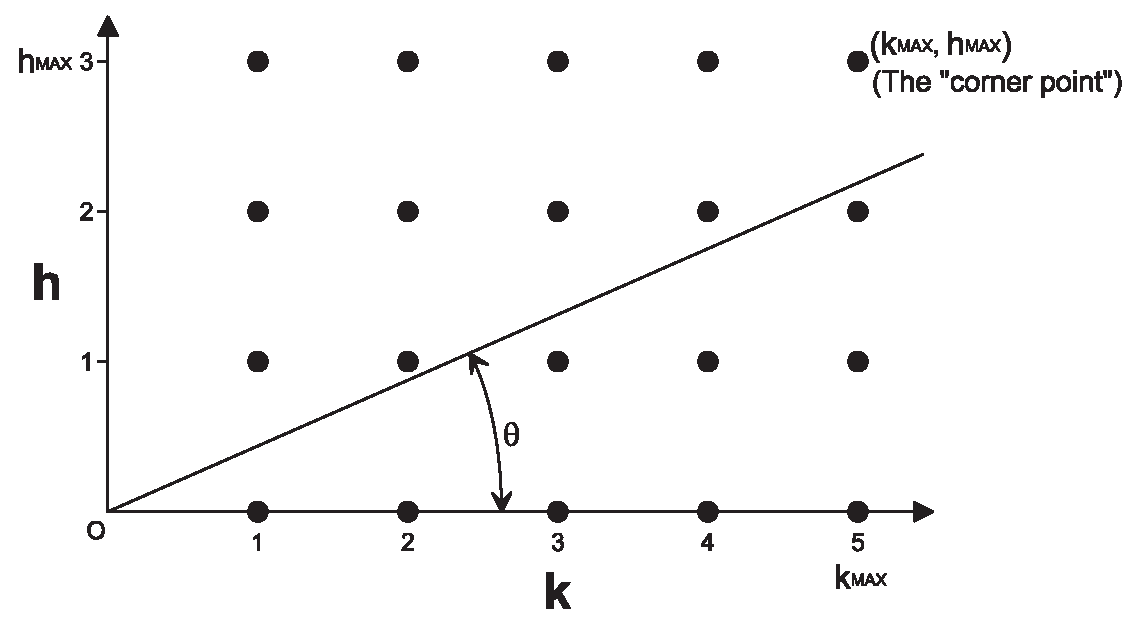
\includegraphics[width=4.6in]{c_fry0/farey01a.eps}
\caption{Graphical Interpretation Of Rational Numbers 
         $h/k$ That Can Be Formed With $h \leq h_{MAX}=3$, $k \leq k_{MAX}=5$}
\label{fig:cfry0:ili0:00}
\end{figure}

From the graphical interpretation suggested by Fig. \ref{fig:cfry0:ili0:00},
the following properties are intuitively clear.

\begin{itemize}
   \item The angle of a ray drawn from the origin to the point
         $(k,h)$ corresponding to the rational number $h/k$ is
         $\theta = tan^{-1} \; h/k$.

   \item Any integer lattice point on a line from 
         the origin drawn at the angle $\theta$
         has the value $h/k = tan \; \theta$.  All points corresponding
         to rational numbers with the same value will be on such a line,
         and thus form an equivalence class.

   \item A rational number $h/k$ is irreducible iff its corresponding
         point $(k,h)$ is ``directly'' visible from the origin with
         no intervening points.

   \item The Farey series of order $N$, $F_N$, can be 
         formed graphically by starting with the
		 set of integer lattice points
		 $(k,h): \; h \in \vworkintsetnonneg \wedge 1 \leq k \leq N$, 
		 then sweeping
         a line extended from the origin, starting with 
         angle $\theta = 0$, through
         $0 \leq \theta < \pi{}/2$, and recording 
         in order each point directly visible from
         the origin.\footnote{Note that Fig. \ref{fig:cfry0:ili0:00},
         because it illustrates the case when $h$ is constrained
         as well, does not show integer lattice points for
         $h > h_{MAX}$.  In principle, if the integer lattice shown
         in Fig. \ref{fig:cfry0:ili0:00} were extended indefinitely
         ``upward'', every positive irreducible rational number with
         $k \leq k_{MAX} = 5$ could be found graphically.}
\end{itemize}

Fig. \ref{fig:cfry0:chk0:01} illustrates the graphical construction method
of $F_5$.  Note that only integer lattice points which are directly
visible from the origin (with no intervening points) are selected.
(Fig. \ref{fig:cfry0:chk0:01}, like Fig. \ref{fig:cfry0:ili0:00},
shows the case of constrained $h$---the integer lattice should be
continued ``upward'' to construct the Farey series.)

\begin{figure}
\centering
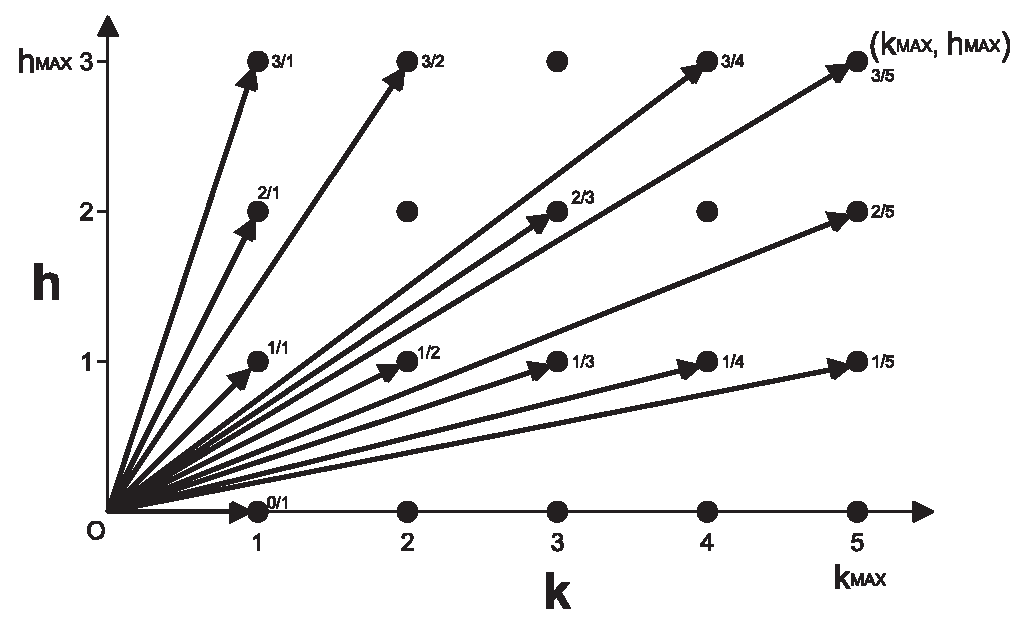
\includegraphics[width=4.6in]{c_fry0/farey01b.eps}
\caption{Graphical Interpretation Of Irreducible Rational Numbers 
         $h/k$ That Can Be Formed With $h \leq h_{MAX}=3$, $k \leq k_{MAX}=5$}
\label{fig:cfry0:chk0:01}
\end{figure}


%%%%%%%%%%%%%%%%%%%%%%%%%%%%%%%%%%%%%%%%%%%%%%%%%%%%%%%%%%%%%%%%%%%%%%%%%%%%%
%%%%%%%%%%%%%%%%%%%%%%%%%%%%%%%%%%%%%%%%%%%%%%%%%%%%%%%%%%%%%%%%%%%%%%%%%%%%%
%%%%%%%%%%%%%%%%%%%%%%%%%%%%%%%%%%%%%%%%%%%%%%%%%%%%%%%%%%%%%%%%%%%%%%%%%%%%%
\section[Generating $F_{k_{MAX}, \overline{h_{MAX}}}$ In A Rectangular Region]
        {Generating \mbox{\boldmath $F_{k_{MAX}, \overline{h_{MAX}}}$}
         Over A Rectangular Region Of The Integer Lattice}
%Section tag: CHK0
\label{cfry0:schk0}

\index{FKMAXHMAX@$F_{k_{MAX}, \overline{h_{MAX}}}$}
In practice, $F_N$ does not represent the set of
rational numbers that may be used for rational approximation in an
application; hence it isn't usually appropriate to choose a
rational number from $F_N$ strictly as
the theory of numbers defines it.  
An actual application is parameterized not just by
$k_{MAX}$ (the maximum denominator that may be chosen, which is considered
in the definition of the Farey series), 
but also by $h_{MAX}$ (the maximum numerator
that may be chosen).  Typically, $h_{MAX}$ exists as a constraint
because a machine multiplication instruction is limited in the size of the
operands it can accomodate; and $k_{MAX}$ exists as a constraint because
a machine division instruction is limited in the size of the divisor
it can accomodate.

In practice, the rational numbers that may be used for rational
approximation represent a rectangular region of the integer
lattice---all $(k,h):$ $h \leq h_{MAX} \wedge k \leq k_{MAX}$ 
(Figs. \ref{fig:cfry0:ili0:00}, \ref{fig:cfry0:chk0:01}).

Fig. \ref{fig:cfry0:ili0:00} supplies a graphical
interpretation of all rational numbers
that can be formed with constraints $h \leq h_{MAX} = 3$ 
and $k \leq k_{MAX} = 5$.  Each point of the integer lattice
shown in the figure is a rational number, not necessarily 
irreducible.  Because under this graphical interpretation
a rational number is irreducible iff it can be reached
by a ray from the origin with no intervening rational numbers,
it is clear that the complete ordered set of irreducible
rational numbers that can be formed under the
constraints $h \leq h_{MAX}$ and $k \leq k_{MAX}$
can be obtained graphically by sweeping a ray from
the origin through the angles $0 \leq \theta < \pi/2$,
recording each point directly visible from the origin.
This graphical construction process is illustrated
in Fig. \ref{fig:cfry0:chk0:01}.

From the graphical construction process shown in 
Fig. \ref{fig:cfry0:chk0:01}, it can be seen that the 
set of irreducible rational numbers that can be formed
subject to the constraints 
$h \leq h_{MAX} \wedge k \leq k_{MAX}$ is:

\begin{equation}
\left\{ { \frac{0}{1}, \frac{1}{5}, \frac{1}{4},
          \frac{1}{3}, \frac{2}{5}, \frac{1}{2},
          \frac{3}{5},
          \frac{2}{3}, \frac{3}{4}, \frac{1}{1},
          \frac{3}{2}, \frac{2}{1}, \frac{3}{1} } \right\} .
\end{equation}

We denote the ordered set of irreducible rational 
numbers that can be formed subject to the
constraints $h \leq h_{MAX} \wedge k \leq k_{MAX}$ as
$F_{k_{MAX}, \overline{h_{MAX}}}$.\footnote{Notationally,
in general,
we use an overbar on the order of a Farey series to
denote that the terms are inverted and reversed in order.
For example, $F_3 = \{ 0/1, 1/3, 1/2, \ldots \}$, but
$F_{\overline{3}}  = \{ \ldots , 2/1, 3/1 \}$.  Notation
such as $F_{A, \overline{B}}$ is an extension of that convention.}

There are three important questions to be asked about
the series $F_{k_{MAX}, \overline{h_{MAX}}}$:

\begin{itemize}
\item What are the smallest and largest rational numbers in
      $F_{k_{MAX}, \overline{h_{MAX}}}$?
      (This question is easy:  the smallest two rational numbers
	  in $F_{k_{MAX}, \overline{h_{MAX}}}$ are $0/1$
	  and $1/k_{MAX}$, and the largest rational number
	  is $h_{MAX}/1$.)

\item How do we construct $F_{k_{MAX}, \overline{h_{MAX}}}$?

\item If we desire to approximate a real number 
      $r_I$, $r_{IMIN} \leq r_I \leq r_{IMAX}$,
      using a rational number selected from 
	  $F_{k_{MAX}, \overline{h_{MAX}}}$, how large might
      the error $| h/k - r_I |$ be?
\end{itemize}


\subsection[Construction Of $F_{k_{MAX},\overline{h_{MAX}}}$]
           {Construction Of \mbox{\boldmath $F_{k_{MAX},\overline{h_{MAX}}}$}}

\index{FKMAXHMAX@$F_{k_{MAX}, \overline{h_{MAX}}}$!construction of}
To construct $F_{k_{MAX}, \overline{h_{MAX}}}$, for 
$0 \leq \theta \leq \tan^{-1} (h_{MAX}/k_{MAX})$---the 
region of the series where $k_{MAX}$ is the dominant constraint,
i.e. below the ``corner point'' in Figs. \ref{fig:cfry0:ili0:00}
and \ref{fig:cfry0:chk0:01}---note
that these terms are simply 
$F_{k_{MAX}}$ up to $h_{MAX}/k_{MAX}$ or its reduced 
equivalent.\footnote{If this is not intuitively clear,
note in Figs. \ref{fig:cfry0:ili0:00} and \ref{fig:cfry0:chk0:01}
that all of the terms of $F_{k_{MAX}}$---that is, all rational
numbers, both reducible and irreducible, with $k \leq k_{MAX}$---are 
available for selection
until the ``corner point'' is reached.}
To construct $F_{k_{MAX}, \overline{h_{MAX}}}$ for
$\tan^{-1} (h_{MAX}/k_{MAX}) < \theta < \pi/2$---the 
region of the series where $h_{MAX}$ is the dominant constraint,
i.e. above the ``corner point'' in Figs. \ref{fig:cfry0:ili0:00}
and \ref{fig:cfry0:chk0:01}---note that by a graphical argument
of symmetry, these terms are the reciprocals of ascending terms of $F_{h_{MAX}}$.
For example, in Fig. \ref{fig:cfry0:chk0:01}, if the $h$- and $k$-
axes are transposed, it is easy to see that $3/1$ in the original integer lattice
would correspond to $1/3$ in the transposed integer lattice.  This argument of
symmetry immediately suggests a procedure for constructing 
$F_{k_{MAX},\overline{h_{MAX}}}$.

\begin{itemize}
\item Construct $F_{k_{MAX}}$ from $0/1$ up through $h_{MAX}/k_{MAX}$ or its
      reduced equivalent.
\item Construct $F_{h_{MAX}}$ from $1/h_{MAX}$ up to $k_{MAX}/h_{MAX}$ or
      its reduced equivalent; then reverse the order of the 
	  terms and take the reciprocal of
      each term.
\item Concatenate the results from the two steps above.
\end{itemize}

\begin{vworkexamplestatement}
\label{ex:cfry0:schk:00}
Construct $F_{5,\overline{3}}$, the set of 
all irreducible rational numbers $h/k$
that can be formed with $h \leq h_{MAX}=3$ and 
$k \leq k_{MAX}=5$.\footnote{Note that $F_{5,\overline{3}}$
is the series depicted in Fig. \ref{fig:cfry0:chk0:01}, and
this example can be verified against the figure.}
\end{vworkexamplestatement}
\begin{vworkexampleparsection}{Solution}
(Using the method of construction presented above.)
First, $F_5$ up through $h_{MAX}/k_{MAX} = 3/5$ or its reduced
equivalent should be constructed.  This series is

\begin{equation}
\label{eq:cfry0:schk:ex00:eq00}
F_5 = 
\left\{ { \frac{0}{1}, \frac{1}{5}, \frac{1}{4},
          \frac{1}{3}, \frac{2}{5}, \frac{1}{2},
          \frac{3}{5}, \ldots{} } \right\} .
\end{equation}

Second, $F_3$ is constructed from $1/3$ up to $k_{MAX}/h_{MAX} = 5/3$ or
its reduced equivalent (not including the
final term, $5/3$).  This series is

\begin{equation}
\label{eq:cfry0:schk:ex00:eq01}
F_3 = 
\left\{ { \ldots , \frac{1}{3}, \frac{1}{2}, \frac{2}{3},
          \frac{1}{1}, \frac{4}{3}, \frac{3}{2}, \ldots{} } \right\} .
\end{equation}

Third, the terms of $F_3$ are reversed in order, and the reciprocal of each term is
calculated, yielding

\begin{equation}
\label{eq:cfry0:schk:ex00:eq02}
F_{\overline{3}} = 
\left\{ { \ldots{}, \frac{2}{3}, \frac{3}{4}, \frac{1}{1},
          \frac{3}{2}, \frac{2}{1}, \frac{3}{1}  } \right\} .
\end{equation}

Finally, concatenating (\ref{eq:cfry0:schk:ex00:eq00})
and
(\ref{eq:cfry0:schk:ex00:eq02}) yields $F_{5,\overline{3}}$, below.

\begin{equation}
\label{eq:cfry0:schk:ex00:eq03}
F_{5,\overline{3}} =
\left\{ { \frac{0}{1}, \frac{1}{5}, \frac{1}{4},
          \frac{1}{3}, \frac{2}{5}, \frac{1}{2},
          \frac{3}{5},
          \frac{2}{3}, \frac{3}{4}, \frac{1}{1},
          \frac{3}{2}, \frac{2}{1}, \frac{3}{1} } \right\}
\end{equation}

\end{vworkexampleparsection}
\vworkexamplefooter{}

It is clear that Thm. \ref{thm:cfry0:sgfs0:01}
and (\ref{eq:cfry0:sgfs0:thm:01:eq01}) through
(\ref{eq:cfry0:sgfs0:thm:01:eq04}) can be used to construct
$F_{k_{MAX}, \overline{h_{MAX}}}$.  However, such algorithms
are not discussed because---even with refinements---they
can be no better than $O(N)$ and are not
fruitful to develop.  Instead, an $O(log N)$
algorithm is presented in 
\ccfrzeroxrefcomma{}\ccfrzeromcclass{} \ref{ccfr0}, 
\emph{\ccfrzeroshorttitle{}}.


%%%%%%%%%%%%%%%%%%%%%%%%%%%%%%%%%%%%%%%%%%%%%%%%%%%%%%%%%%%%%%%%%%%%%%%%%%%%%
%%%%%%%%%%%%%%%%%%%%%%%%%%%%%%%%%%%%%%%%%%%%%%%%%%%%%%%%%%%%%%%%%%%%%%%%%%%%%
%%%%%%%%%%%%%%%%%%%%%%%%%%%%%%%%%%%%%%%%%%%%%%%%%%%%%%%%%%%%%%%%%%%%%%%%%%%%%
\subsection[Distance Between Terms Of $F_{h_{MAX},k_{MAX}}$]
           {Distance Between Terms Of \mbox{\boldmath $F_{h_{MAX},k_{MAX}}$}}

\index{FKMAXHMAX@$F_{k_{MAX}, \overline{h_{MAX}}}$!distance between terms}
\index{Farey series!distance between terms}
The maximum \emph{distance} between terms of $F_{h_{MAX},k_{MAX}}$ also establishes
what we call the maximum \emph{placement error}, $|r_A - r_I|$, in choosing
$r_A = h/k$.  Specifically, the maximum distance is twice the maximum placement
error.  Clearly, with a maximum distance specified, choosing $r_I = (x+y)/2$ for
two successive terms $x$ and $y$ separated by the maximum distance is 
the most antagonistic
choice of $r_I$ possible.
We use the two notions (maximum distance and maximum placement error)
interchangeably and don't bother to convert between them, as they are
the same notion and differ only by a factor of two.

It is clear from the earlier discussion of the Farey series that the maximum
distance between terms in $F_{k_{MAX}}$ is $1/k_{MAX}$, and that this maximum
distance occurs only adjacent to an integer.  It is also clear from the
discussion of $F_{\overline{h_{MAX}}}$ that the maximum distance between terms
is 1.

Thus, when we use $F_{k_{MAX}, \overline{h_{MAX}}}$ to approximate real numbers,
in general the worst-case distance between terms is 1.

In practical applications when rational approximation is used,
the approximation tends to be used over a restricted interval
$[l \gg  0, r \ll h_{MAX}]$ rather than over the full range of the rational numbers that
can be formed, $[0, h_{MAX}]$.  This section develops novel upper bounds on
the distance between terms of $F_{k_{MAX}, \overline{h_{MAX}}}$ in an interval
$[l,r]$.  For simplicity, assume $l,r \in F_{k_{MAX}, \overline{h_{MAX}}}$.

Three distinct cases are developed (Figure \ref{fig:cfry0:schk0:threecases}).
The upper bound developed from Case III is always larger than the upper
bound developed from Case II, which is always larger than the upper bound developed
from Case I; so if only the absolute maximum error over
the interval $[l,r]$ is of interest, only the
highest-numbered case which applies needs to be evaluated.  However, some
applications may have different error requirements in different regions
of the interval $[l,r]$, and for these applications it may be beneficial
to analyze more than one case.

\begin{figure}
\centering
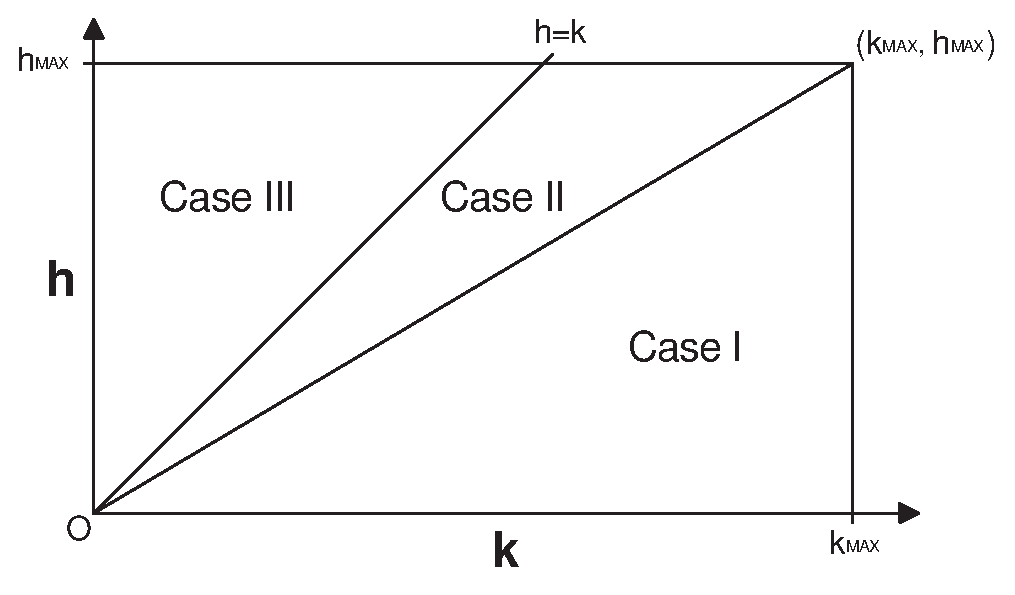
\includegraphics[width=4.6in]{c_fry0/errreg01.eps}
\caption{Three Cases For Bounding Distance Between Terms In 
         $F_{k_{MAX}, \overline{h_{MAX}}}$}
\label{fig:cfry0:schk0:threecases}
\end{figure}


\subsubsection[Case I:  $r_I < h_{MAX}/k_{MAX}$]
              {Case I:  \mbox{\boldmath $r_I < h_{MAX}/k_{MAX}$}}

With $r_I < h_{MAX}/k_{MAX}$, $k \leq k_{MAX}$ is the dominant
constraint, and the neighbors available to $r_I$ are simply the
terms of $F_{k_{MAX}}$.  If $[l, r] \cap  [0, h_{MAX}/k_{MAX}]$
includes an integer, clearly the maximum distance from $r_I$ to the
nearest available term of $F_{k_{MAX}, \overline{h_{MAX}}}$ is given
by

\begin{equation}
\left|
\frac{h}{k} - r_I
\right|
\leq
\frac{1}{2 k_{MAX}} ,
\end{equation}

which is the same result for the Farey series in general.

If $[l, r] \cap  [0, h_{MAX}/k_{MAX}]$ does
not include an integer, it can be shown that the
maximum distance between Farey terms is driven by the
rational number with the smallest denominator in the
interval $[l, r]$.

For two consecutive terms $p/q$ and $p'/q'$ in $F_{k_{MAX}}$,
$p'q - pq' = 1$ (Thm. \ref{thm:cfry0:spfs:02}), so that

\begin{equation}
\frac{p'}{q'} - \frac{p}{q} =
\frac{p'q - pq'}{q q'} = \frac{1}{qq'} .
\end{equation}

By Thm. \ref{thm:cfry0:spfs:02ba}, $q+q' > k_{MAX}$, therefore

\begin{equation}
\label{eq:cfry0:schk0:minqplacementupperbound}
\frac{1}{q k_{MAX}} \leq
\frac{1}{q q'} <
\frac{1}{q (k_{MAX}-q)}.
\end{equation}

Let $q_{MIN}$ be the smallest denominator of any rational number
$\in F_{k_{MAX}}$ in the interval $[l,r]$.  It is then easy to show
that for any consecutive denominators $q, q'$ which occur in
$F_{k_{MAX}}$ in the interval $[l,r]$,

\begin{equation}
\frac{1}{q q'} < \frac{1}{q_{MIN} \; max (q_{MIN}, k_{MAX} - q_{MIN})} .
\end{equation}

Thus, the upper bound on the distance between consecutive terms of $F_{k_{MAX}}$
in an interval $[l,r]$ is tied to the minimum denominator of any
rational number $\in F_{k_{MAX}}$ in $[l,r]$.

Note that clearly
$q_{MIN} \leq 1/(r-l)$, so for most practical intervals $[l,r]$,
the search for $q_{MIN}$ would not be computationally expensive.
However, applications could arise where an approximation is used
in an \emph{extremely} narrow interval, and having an algorithm available that
is computationally viable for such cases is advantageous.  For example,
locating the rational number $\in F_{2^{20,000}}$ with the smallest denominator
in an interval of width $2^{-10,000}$ could be a serious computational
problem.

To locate $q_{MIN}$ in $[l,r]$, note that at least one rational number
with $q_{MIN}$ as a denominator in $[l,r]$ is the best approximation
of order $q_{MIN}$ to the midpoint of the interval,
$(l+r)/2$.\footnote{Thanks to David M. Einstein \cite{bibref:i:davidmeinstein} 
and David Eppstein \cite{bibref:i:davideppstein}
for this observation, contributed via the \texttt{sci.math} newsgroup
\cite{bibref:n:scimathnewsgroup},
which is the linchpin of Algorithm \ref{alg:cfmindenominator}.}
By theorem (\cite{bibref:b:KhinchinClassic}, Theorem 15), every best approximation
of a number is a convergent or intermediate fraction of the
continued fraction representation of the number.  We seek the
convergent or intermediate fraction of $(l+r)/2$ with the smallest
denominator that is in the interval $[l,r]$.\footnote{Regrettably,
at this point the cart comes before the horse---the insight and
algorithms which follow are based on continued fractions, which
are not covered until \ccfrzeroxrefcomma{}\ccfrzeromcclass{} \ref{ccfr0}, 
\emph{\ccfrzeroshorttitle{}}.  We apologize for the potential necessity
of reading this work out of order.}

The convergents and intermediate fractions of $(l+r)/2$ are naturally
arranged in order of increasing denominator.  However, it would be
inefficient to test \emph{every} intermediate fraction
for membership in $[l,r]$, as partial quotients $a_k$ are unlimited in
size and such an algorithm may not be $O(log \; k_{MAX})$.  Instead,
since intermediate fractions are formed using the parameterized
expression $(i p_k + p_{k-1})/(i q_k + q_{k-1})$,
and since intermediate fractions are ever-increasing
or ever-decreasing with respect to the parameter $i$, the
smallest value of $i$ which will create an intermediate
fraction potentially within $[l,r]$ can be directly
calculated.  Only the intermediate fraction formed with
this calculated value of $i$ needs to be tested for membership in
$[l,r]$.

Let $l_N$ and $l_D$ be the numerator and denominator of $l$, and
let $r_N$ and $r_D$ be the numerator and denominator of $r$.
In the case of $k$ even; $s_k < l < (l+r)/2$ (otherwise $s_k$
would have been identified as $\in [l,r]$, see Algorithm
\ref{alg:cfmindenominator}); $s_{k+1} \geq (l+r)/2$;
with increasing $i$, $(i p_k + p_{k-1})/(i q_k + q_{k-1})$
forms a decreasing sequence; and the inequality we seek to solve is

\begin{equation}
\label{eq:cfry0:schk0:ifselection01}
\frac{i p_k + p_{k-1}}{i q_k + q_{k-1}} \leq \frac{r_N}{r_D}.
\end{equation}

Solving (\ref{eq:cfry0:schk0:ifselection01}), the smallest integral 
value of $i$ that will suffice is

\begin{equation}
\label{eq:cfry0:schk0:ifselection02}
i = \left\lceil {
\frac{r_N q_{k-1} - r_D p_{k-1}}{r_D p_k - r_N q_k}
} \right\rceil .
\end{equation}

Similarly, for $k$ odd, the sequence is increasing,
and the inequality and solution are

\begin{equation}
\label{eq:cfry0:schk0:ifselection03}
\frac{i p_k + p_{k-1}}{i q_k + q_{k-1}} \geq \frac{l_N}{l_D}
\to
i = \left\lceil {
\frac{l_N q_{k-1} - l_D p_{k-1}}{l_D p_k - l_N q_k}
} \right\rceil .
\end{equation}

(\ref{eq:cfry0:schk0:ifselection01}),
(\ref{eq:cfry0:schk0:ifselection02}),
and (\ref{eq:cfry0:schk0:ifselection03}) suggest the following continued fraction
algorithm for finding
a rational number with the smallest denominator in an
interval $[l,r]$.

\begin{vworkalgorithmstatement}\label{alg:cfmindenominator}\end{vworkalgorithmstatement}
\begin{alglvl0}
\item Calculate all partial quotients $a_k$ and all convergents
      $s_k = p_k/q_k$ of the midpoint of the interval,
      $(l+r)/2$.

\item  For each convergent $s_k=p_k/q_k$, in order of increasing $k$:

   \begin{alglvl1}

   \item If $s_k = p_k/q_k \in [l,r]$, $s_k$ is a rational number with
         the lowest denominator, STOP.

   \item If $k$ is even,

      \begin{alglvl2}

      \item Calculate $i$ according to (\ref{eq:cfry0:schk0:ifselection02}).
            If $i < a_{k+1}$ and the intermediate fraction
            $(i p_k + p_{k-1})$ $/$ $(i q_k + q_{k-1})$ $\geq$ $l$, this intermediate
            fraction is
            a rational number with the lowest denominator, STOP.

      \end{alglvl2}

   \item Else if $k$ is odd,

      \begin{alglvl2}

      \item Calculate $i$ according to (\ref{eq:cfry0:schk0:ifselection03}).
            If $i < a_{k+1}$ and the intermediate fraction
            $(i p_k + p_{k-1})$ $/$ $(i q_k + q_{k-1})$ $\leq$ $r$, this intermediate
            fraction is
            a rational number with the lowest denominator, STOP.

      \end{alglvl2}

   \end{alglvl1}

\end{alglvl0}

Algorithm \ref{alg:cfmindenominator} is approximately $O(log \; k_{MAX})$,
since there are a fixed number of steps per convergent, and the maximum number
of convergents is $O(log \; k_{MAX})$.  Once a rational number with the smallest
denominator $q_{MIN}$ is located, (\ref{eq:cfry0:schk0:minqplacementupperbound})
can be applied to bound $|r_A - r_I|$; namely,

\begin{equation}
\label{eq:qminmaxplacementerror}
\left| {\frac{h}{k} - r_I}  \right|
<
\frac{1}{2q_{MIN} \; max(q_{MIN}, k_{MAX} - q_{MIN})} .
\end{equation}


%%%%%%%%%%%%%%%%%%%%%%%%%%%%%%%%%%%%%%%%%%%%%%%%%%%%%%%%%%%%%%%%%%%%%%%%%%%%%
%%%%%%%%%%%%%%%%%%%%%%%%%%%%%%%%%%%%%%%%%%%%%%%%%%%%%%%%%%%%%%%%%%%%%%%%%%%%%
%%%%%%%%%%%%%%%%%%%%%%%%%%%%%%%%%%%%%%%%%%%%%%%%%%%%%%%%%%%%%%%%%%%%%%%%%%%%%
\subsubsection[Case II:  $h_{MAX}/k_{MAX} < r_I < 1$]
              {Case II:  \mbox{\boldmath $h_{MAX}/k_{MAX} < r_I < 1$}}

If $h_{MAX}/k_{MAX} < r_I < 1$, a graphical argument
(Figure \ref{fig:cfry0:schk0:caseii}) can be used
to more tightly bound the maximum distance between terms of
$F_{k_{MAX}, \overline{h_{MAX}}}$.

\begin{figure}
\centering
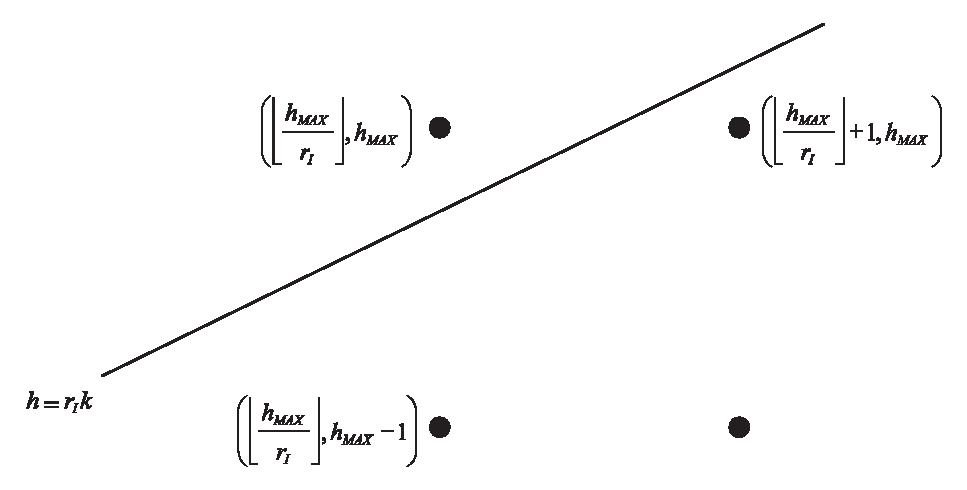
\includegraphics[height=2.0in]{c_fry0/errcase2.eps}
\caption{Graphical Interpretation Of Case II:  $h_{MAX}/k_{MAX} < r_I < 1$}
\label{fig:cfry0:schk0:caseii}
\end{figure}

In this case,  a formable term at or to the left\footnote{To the left on the
number line, but to the right in Figure \ref{fig:cfry0:schk0:caseii}.}
of $r_I$ is represented by the point $(\lfloor h_{MAX}/r_I \rfloor + 1, h_{MAX} )$
in the integer lattice,
and a formable term at or to the right of $r_I$ is
represented by the point $(\lfloor h_{MAX}/r_I \rfloor, h_{MAX} )$
in the integer lattice.  Thus, the maximum distance between
neighboring terms in $F_{k_{MAX}, \overline{h_{MAX}}}$
is given by the difference of these two terms,

\begin{equation}
\frac{h_{MAX}}{\left\lfloor {\frac{h_{MAX}}{r_I}} \right\rfloor}
-
\frac{h_{MAX}}{\left\lfloor {\frac{h_{MAX}}{r_I}} \right\rfloor + 1}
=
\frac{h_{MAX}}{{\left\lfloor {\frac{h_{MAX}}{r_I}} \right\rfloor}^2
+ \left\lfloor {\frac{h_{MAX}}{r_I}} \right\rfloor},
\end{equation}

and the maximum distance from $r_I$ to a neighboring term is
given by

\begin{equation}
\label{eq:cfry0:schk0:caseiimaxplacementerror}
\left|
\frac{h}{k} - r_I
\right|
\leq
\frac{h_{MAX}}{2 \left( { {\left\lfloor {\frac{h_{MAX}}{r_I}} \right\rfloor}^2
+ \left\lfloor {\frac{h_{MAX}}{r_I}} \right\rfloor } \right) }.
\end{equation}

Note that Case II will exist only if $h_{MAX}/k_{MAX} < 1$.


\subsubsection[Case III:  $1 < h_{MAX}/k_{MAX} < r_I$]
              {Case III:  \mbox{\boldmath $1 < h_{MAX}/k_{MAX} < r_I$}}

It can be established graphically, using the coordinate system of
Figure \ref{fig:cfry0:ili0:00}, Figure \ref{fig:cfry0:chk0:01},
or Figure \ref{fig:cfry0:schk0:threecases}, 
that the line $h=r_I k$ intercepts the
line $h=h_{MAX}$ at the point $(h_{MAX}/r_I, h_{MAX})$.  It is clear
from a graphical argument that all of the terms of the Farey series
of order $\lfloor h_{MAX}/r_I \rfloor$ are available as neighbors
of $r_I$.  Therefore,

\begin{equation}
\label{eq:cfry0:schk0:caseiiiplacementerror}
\left|
\frac{h}{k} - r_I
\right|
\leq
\frac{1}{2 \left\lfloor \frac{h_{MAX}}{r_I} \right\rfloor}.
\end{equation}


%%%%%%%%%%%%%%%%%%%%%%%%%%%%%%%%%%%%%%%%%%%%%%%%%%%%%%%%%%%%%%%%%%%%%%%%%%%%%
%%%%%%%%%%%%%%%%%%%%%%%%%%%%%%%%%%%%%%%%%%%%%%%%%%%%%%%%%%%%%%%%%%%%%%%%%%%%%
%%%%%%%%%%%%%%%%%%%%%%%%%%%%%%%%%%%%%%%%%%%%%%%%%%%%%%%%%%%%%%%%%%%%%%%%%%%%%
\section{Acknowledgements}
%Section tag: ACK0

This chapter is the result of work on inexpensive microcontroller 
arithmetic (and a paper) undertaken in 2000.
We would like to gratefully acknowledge the assistance
of 
\index{Bachelis, Greg}      Greg Bachelis     \cite{bibref:i:gregbachelis}, 
\index{Berman, Robert}      Robert Berman     \cite{bibref:i:robertberman}, 
\index{Lin, Feng}           Feng Lin          \cite{bibref:i:fenglin}, 
\index{Sahinidis, Nick}     Nick Sahinidis    \cite{bibref:i:nicksahinidis}, 
\index{Van Tuyl, Adam}      Adam Van Tuyl     \cite{bibref:i:adamvantuyl},
\index{Schweiger, Carl}     Carl Schweiger    \cite{bibref:i:carlschweiger}, 
\index{Tindell, Ken}        Ken Tindell       \cite{bibref:i:kentindell},
\index{Vestal, Steve}       Steve Vestal      \cite{bibref:i:stevevestal},
\index{Whitinger, Bob}      Bob Whitinger     \cite{bibref:i:bobwhitinger},
and 
\index{Stewart, David B.}   David B. Stewart   \cite{bibref:i:davidbstewart}
in finding the areas of
mathematics relevant to the rational number selection
problem.  We would also like to
thank 
\index{Bengtsson, Johan}    Johan Bengtsson    \cite{bibref:i:johanbengtsson},
\index{Burke, Michael J.}   Michael J. Burke   \cite{bibref:i:michaeljburke},  
\index{Endicott, Mark}      Mark Endicott      \cite{bibref:i:markendicott}, 
\index{Eppstein, David}     David Eppstein     \cite{bibref:i:davideppstein}, 
\index{Munteanu, Mircea}    Mircea Munteanu    \cite{bibref:i:mirceamunteanu},
\index{Gibson, Adam}        Adam Gibson        \cite{bibref:i:adamgibson}, 
and \index{Virgil}          Virgil             \cite{bibref:i:virgil}
(of the \index{sci.math.num-analysis@\texttt{sci.math.num-analysis} newsgroup}%
\texttt{sci.math.num-analysis} newsgroup 
\cite{bibref:n:scimathnumanalysis})
for insight into this problem; 
\index{Stallings, Cliff}    Cliff Stallings    \cite{bibref:i:cliffstallings}
and
\index{Kakos, Robert}       Robert Kakos       \cite{bibref:i:robertkakos}
for support from Wayne State
University's College Of Engineering; 
\index{Groen, Paulette}     Paulette Groen     \cite{bibref:i:paulettegroen}
and
\index{Smith, Paula}        Paula Smith        \cite{bibref:i:paulasmith}
for support from \index{Visteon}Visteon;
\index{Crosby, Bob}         Bob Crosby         \cite{bibref:i:bobcrosby}
for support
from \index{Texas Instruments}Texas Instruments; 
\index{Zauner, Klaus-Peter} Klaus-Peter Zauner  \cite{bibref:i:klauspeterzauner},
\index{Blome, Andrea}       Andrea Blome        \cite{bibref:i:andreablome},
\index{Smith, Una}          Una Smith           \cite{bibref:i:unasmith},
\index{Tinnefeld, Karsten}  Karsten Tinnefeld   \cite{bibref:i:karstentinnefeld},
and
\index{Franke, Axel}        Axel Franke         \cite{bibref:i:axelfranke}
for other tool
and logistical support; and the management
team at Visteon for allowing us to pursue this
effort in the workplace.


%%%%%%%%%%%%%%%%%%%%%%%%%%%%%%%%%%%%%%%%%%%%%%%%%%%%%%%%%%%%%%%%%%%%%%%%%%%%%
%%%%%%%%%%%%%%%%%%%%%%%%%%%%%%%%%%%%%%%%%%%%%%%%%%%%%%%%%%%%%%%%%%%%%%%%%%%%%
%%%%%%%%%%%%%%%%%%%%%%%%%%%%%%%%%%%%%%%%%%%%%%%%%%%%%%%%%%%%%%%%%%%%%%%%%%%%%
\section{Exercises}
%Section tag: EXE0

\begin{vworkexercisestatement}
\label{exe:cfry0:sexe0:01}
Prove that Theorem \ref{thm:cfry0:spfs:01}
holds in the degenerate cases where $h=1$ and where $k=1$.
\end{vworkexercisestatement}
\vworkexercisefooter{}

\begin{vworkexercisestatement}
\label{exe:cfry0:sexe0:02}
Prove that Theorem \ref{thm:cfry0:spfs:01} holds $\forall i \in \vworkintset$
(rather than $\forall i \in \vworkintsetnonneg$) using
the slightly amended notion of reducibility that $h/k$ is irreducible iff
$\lfloor h \rfloor / k$ is irreducible.
\end{vworkexercisestatement}
\vworkexercisefooter{}

\begin{vworkexercisestatement}
In Section \ref{cfry0:sgfs0} and Algorithm \ref{alg:cfry0:sgfs0:02}
it is stated that for $i \in \vworkintsetnonneg$, 
$(iN-1)/N$, $i/1$, and $(iN+1)/N$ are consecutive terms in the Farey series
or order $N$, $F_N$.  Prove that $(iN-1)/N$ and $(iN+1)/N$ are irreducible,
and the left and right Farey neighbors to $i/1$.
\end{vworkexercisestatement}
\vworkexercisefooter{}

\begin{vworkexercisestatement}
Prove that in $F_N$ the maximum distance between terms $1/N$ can occur
only adjacent to an integer.
\end{vworkexercisestatement}
\vworkexercisefooter{}


%%%%%%%%%%%%%%%%%%%%%%%%%%%%%%%%%%%%%%%%%%%%%%%%%%%%%%%%%%%%%%%%%%%%%%%%%%

\noindent\begin{figure}[!b]
\noindent\rule[-0.25in]{\textwidth}{1pt}
\begin{tiny}
\begin{verbatim}
$HeadURL: svn://localhost/dtapublic/pubs/books/ucbka/trunk/c_fry0/c_fry0.tex $
$Revision: 277 $
$Date: 2019-08-12 22:35:39 -0400 (Mon, 12 Aug 2019) $
$Author: dashley $
\end{verbatim}
\end{tiny}
\noindent\rule[0.25in]{\textwidth}{1pt}
\end{figure}

%%%%%%%%%%%%%%%%%%%%%%%%%%%%%%%%%%%%%%%%%%%%%%%%%%%%%%%%%%%%%%%%%%%%%%%%%%
%
%End of file C_FRY0.TEX
